\begin{flushleft}
	\section{\textcolor{cyan}{Les Outils logiciels utilisés dans le projet}}
	\subsection{\textcolor{green}{Firebase :}}
	\begin{figure}[h]
		\begin{minipage}{0.6\textwidth}
			Firebase est une plateforme de développement d'applications mobiles et web, initialement développée par Firebase, Inc. et acquise par Google en 2014. Elle fournit une variété d'outils et de services, notamment une base de données en temps réel, une authentification, un hébergement, des messages cloud, des fonctions cloud, des analyses, et bien plus encore. Firebase est connue pour sa facilité d'utilisation, sa scalabilité et sa flexibilité, ce qui en fait un choix populaire pour les développeurs qui souhaitent créer des applications web et mobiles. Elle fournit également une documentation robuste, un support étendu et une communauté active pour aider les développeurs à résoudre les problèmes qu'ils peuvent rencontrer.
		\end{minipage}
		\begin{minipage}{0.4\textwidth}
			\centering
			
\includegraphics[width=\textwidth]{chapitres/images/firebase.png}
			\caption{Firebase}
			\label{fig:votre_image}
		\end{minipage}
	\end{figure}
	\subsection{\textcolor{green}{Flutter et VS Code :}}
	\begin{figure}[h]
		\begin{minipage}{0.6\textwidth}
			Flutter est un framework open-source créé par Google pour le développement d'applications mobiles pour Android et iOS. VS Code est un éditeur de code open-source créé par Microsoft.
			
			Flutter peut être utilisé avec différents éditeurs de code, mais VS Code est un choix populaire pour le développement Flutter car il fournit un support intégré pour le développement Flutter. VS Code fournit des fonctionnalités telles que l'autocomplétion, la refactorisation, le débogage et l'intégration avec les outils de gestion de version.
			
			Avec l'extension Flutter pour VS Code, les développeurs peuvent facilement créer de nouveaux projets Flutter, ajouter des packages, exécuter des tests, déboguer des erreurs et publier leurs applications directement depuis VS Code. En outre, VS Code fournit une grande communauté d'utilisateurs et de développeurs, ce qui facilite le partage de connaissances et de ressources.
			
			En résumé, Flutter et VS Code sont deux technologies complémentaires pour le développement d'applications mobiles, et leur utilisation ensemble offre un environnement de développement efficace et productif.
		\end{minipage}
		\begin{minipage}{0.4\textwidth}
			\centering
			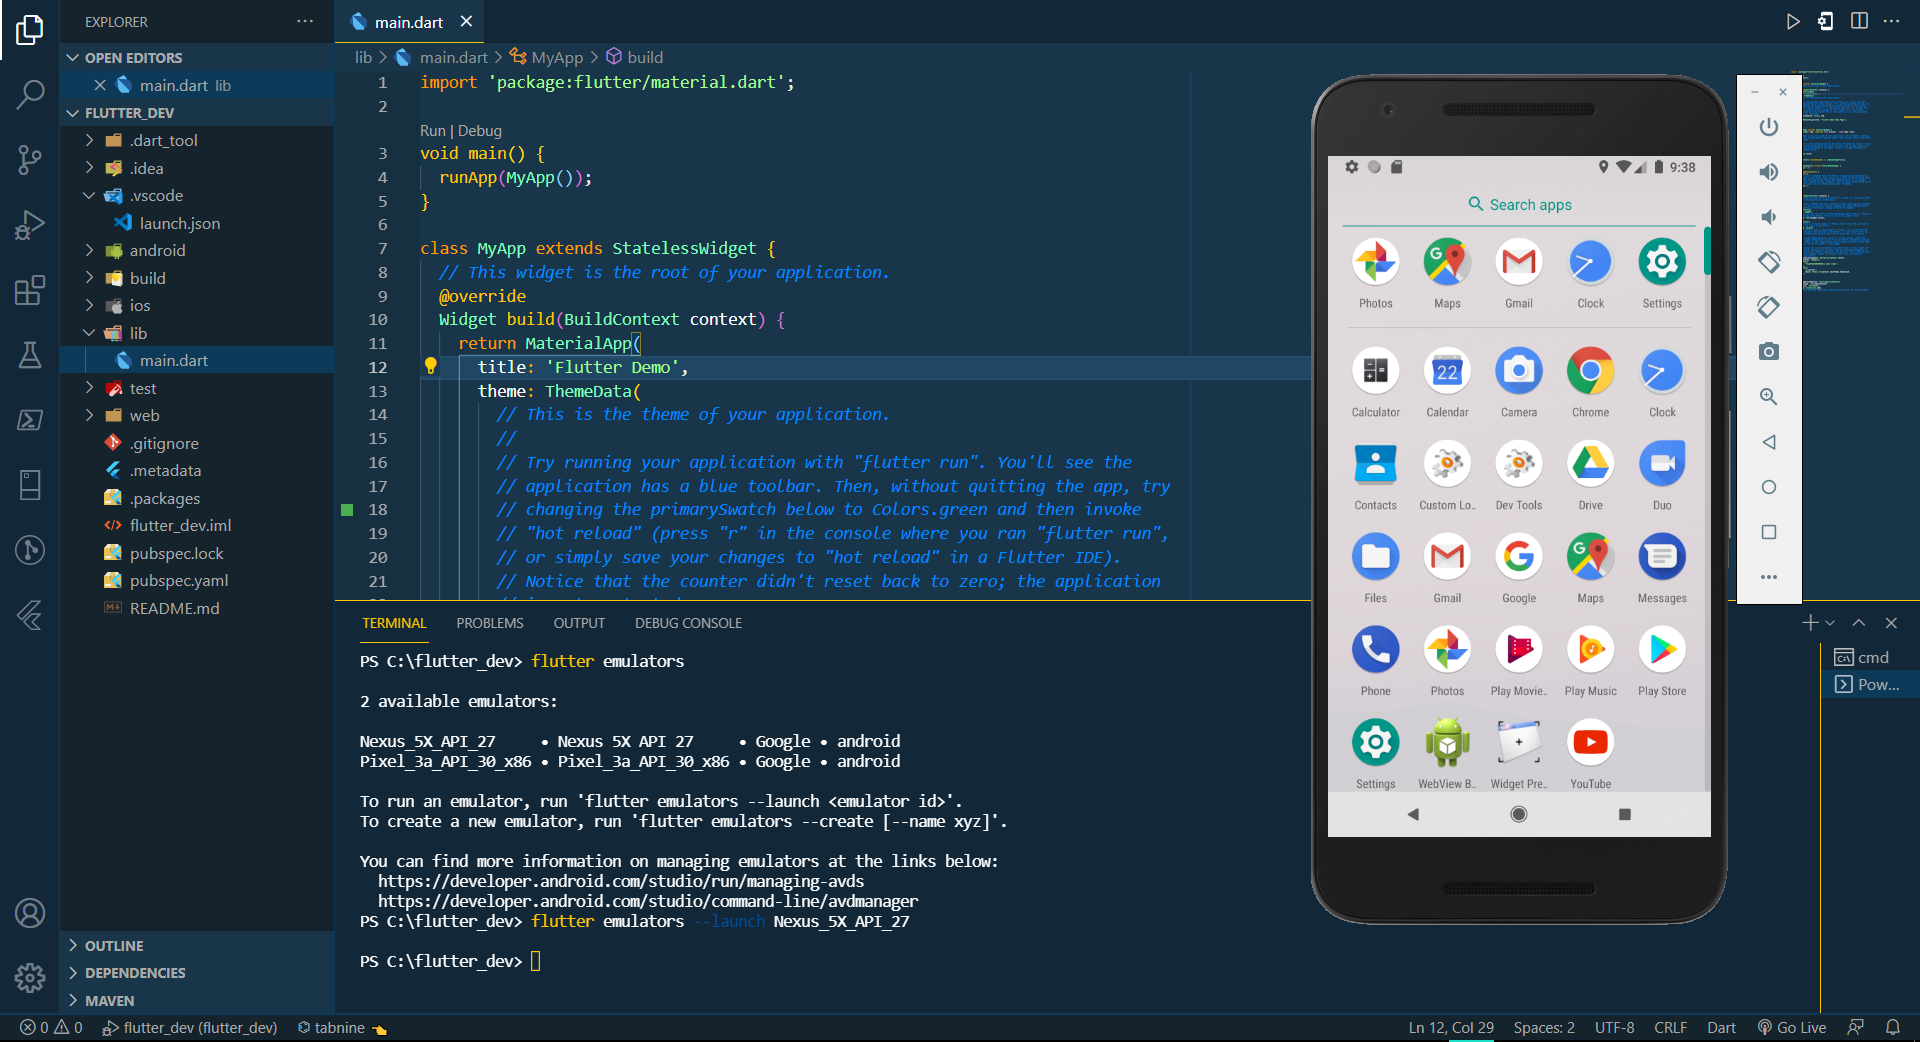
\includegraphics[width=\textwidth]{chapitres/images/flutterVSCode.png}
			\caption{Flutter et VS Code}
			\label{fig:votre_image}
		\end{minipage}
	\end{figure}
	\subsection{\textcolor{green}{Arduino IDE :}}
	\begin{figure}[h]
		\begin{minipage}{0.6\textwidth}
			Arduino IDE est un environnement de développement intégré (IDE) open-source conçu pour programmer les cartes Arduino. Les cartes Arduino sont des microcontrôleurs programmables qui peuvent être utilisés pour contrôler divers appareils électroniques.
			
			L'IDE Arduino fournit une interface utilisateur graphique conviviale pour écrire, compiler et téléverser des programmes vers la carte Arduino. Il prend en charge une grande variété de langages de programmation, y compris le langage de programmation Arduino, qui est basé sur C++.
			
			L'IDE Arduino inclut également une bibliothèque de fonctions standard qui peut être utilisée pour contrôler les entrées et sorties de la carte Arduino, tels que les ports analogiques et numériques, les boutons-poussoirs, les capteurs, les LED, les moteurs et plus encore. Il existe également de nombreuses bibliothèques tierces disponibles pour ajouter des fonctionnalités supplémentaires à vos projets Arduino.
			
			En somme, l'IDE Arduino est une plate-forme de développement très populaire pour les débutants et les experts en électronique qui souhaitent programmer des cartes Arduino et créer des projets électroniques personnalisés.
		\end{minipage}
		\begin{minipage}{0.4\textwidth}
			\centering
			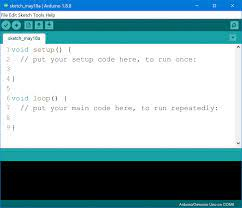
\includegraphics[width=\textwidth]{chapitres/images/aruinoIDE.jpg}
			\caption{Arduino IDE}
			\label{fig:votre_image}
		\end{minipage}
	\end{figure}
	
	\newpage
\end{flushleft}